\section{Expected Utilization with $R_{on}$, $T_{on}$, and $T_{off}$ as 
Random Variables}
  In this section we study the expected utilization when treating $R_{on}$, 
  $T_{on}$, and $T_{off}$ as random variables and fixing the value of 
  $RTT$. Figure \ref{taueta} plots the expected utilization as a function of 
  $\tau - \eta$. In Figure \ref{taueta}, $C = 1Gbps$, $RTT = 100ms$, $\tau \in 
  \{50ms, 500ms, 1s\}$, $\eta$ is varied over $[1ms, \tau]$, $E[T_{on}] \in 
  \{25ms, 100ms\}$, $E[T_{off}] \in \{25ms, 100ms\}$, and $E[R_{on}] \in 
  \{125Mbps, 375Mbps, \\ 500Mbps\}$. The probability density functions of 
  $R_{on}$, $T_{on}$, and $T_{off}$ are defined as follows:
  \begin{IEEEeqnarray}{rCl}
    f_{T_{on}}(T_{on}) & = &
    \begin{cases}
      \frac{1}{0.04} & \text{if } E[T_{on}] - 0.02 < T_{on} < E[T_{on}] + 
      0.02 \\
      0 & \text{otherwise}
    \end{cases}
    \label{tonpdf} \\
    f_{T_{off}}(T_{off}) & = &
    \begin{cases}
      \frac{1}{0.04} & \text{if } E[T_{off}] - 0.02 < T_{off} < E[T_{off}] + 
      0.02 \\
      0 & \text{otherwise}
    \end{cases}
    \label{toffpdf} \\
    f_{R_{on}}(R_{on}) & = &
    \begin{cases}
      \frac{2}{C} & \text{if } \frac{C}{2} < R_{on} < C \\
      0 & \text{otherwise}
    \end{cases}
    \label{ronpdf}
  \end{IEEEeqnarray} 

  As with random $RTT$, we observe that:
  \begin{itemize}
    \item The expected utilization decreases with increasing $\tau - \eta$.
    \item For large $\tau - \eta$, the performance of Rapid is slightly 
    affected.
    \item For a given value of $\tau - \eta$, Rapid performs better of larger 
    values of $\tau$.
  \end{itemize}

  \begin{figure}[!htb]
    \centering
    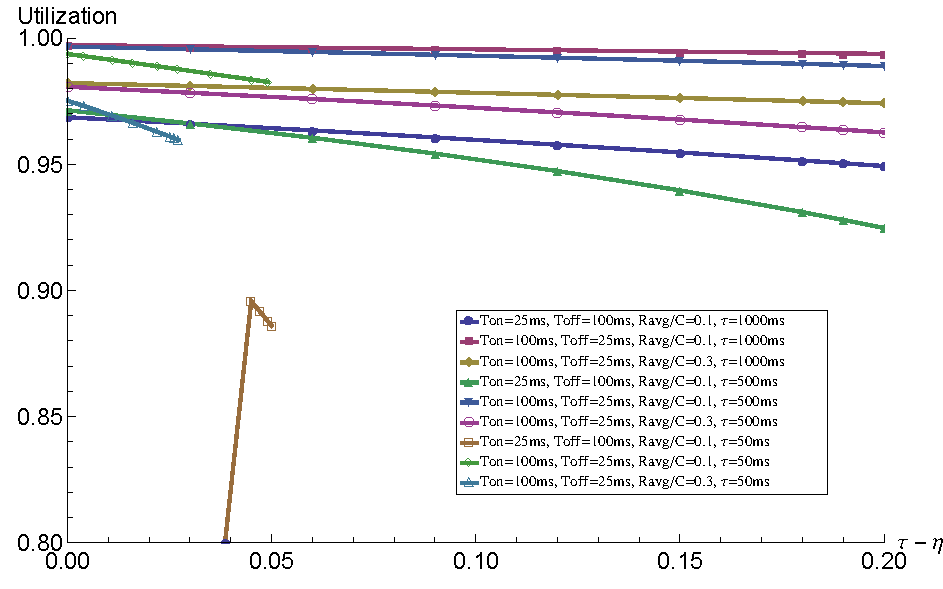
\includegraphics[width=0.9\textwidth]{img/taueta.pdf}
    \caption{Role of $\tau - \eta$}
    \label{taueta}
  \end{figure}

  Figure \ref{comparison} compares the worst case utilization, the expected 
  utilization with random $RTT$, and the expected utilization with random 
  $T_{on}$, $T_{off}$, and $R_{on}$. We observe that Rapid performance is 
  better when treating $T_{on}$, $T_{off}$, and $R_{on}$ as random variables.
  The same result is obtained when comparing Rapid performance with other 
  combination of values.
  \begin{figure}[!htb]
    \centering
    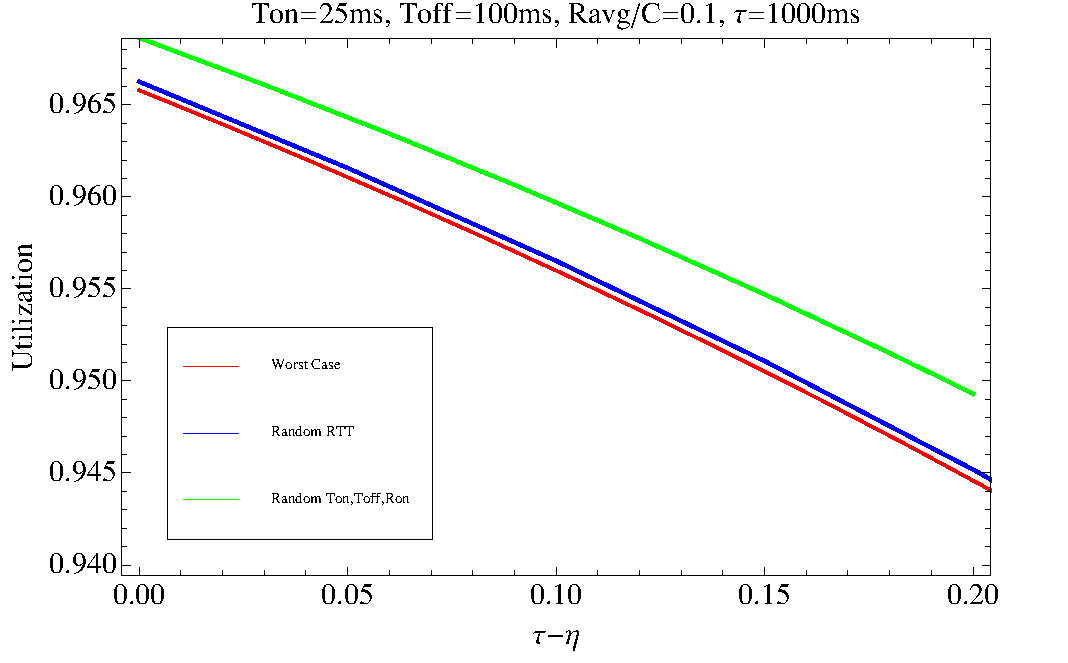
\includegraphics[width=0.9\textwidth]{img/comparison.pdf}
    \caption{Wost case utilization and expected utilization}
    \label{comparison}
  \end{figure}

